\Tr
\twocolumn[\begin{center}{\red More neutrino data needed at multi-PeV energies}\end{center}]
\begin{itemize}
\item[] \colorbox{yellow}{Radio signals of $\nu$ showers}
\item Long (km-scale) attenuation length
\item[] Cover large ($\sim$200 km$^{2}$) area
\item {\blue Detect events $>10^{17}$ eV}
\item \colorbox{yellow}{GZK $\nu$ : Proof of GZK effect}
\item[] or : \colorbox{yellow}{Insight in UHECR composition}
\item $p+\gamma \rightarrow \Delta \rightarrow \nu \quad (E_{\nu} \approx 4\%~E_{p})$
\item[] $p+\gamma_{EBL}$ : Low-E bump
\item[] $p+\gamma_{CMB}$ : High-E bump
\item Iron: lower $E/A$ and dissociation
\item[] $\rightarrow$ Higher $E$ threshold and lower flux
\item {\blue IceCube-Radio energy gap}
\item[] Currently not covered
\end{itemize}

\newpage

\begin{center}
{\blue The multi-PeV neutrino landscape}\\
{\large [arXiv:1802.05543]}\\
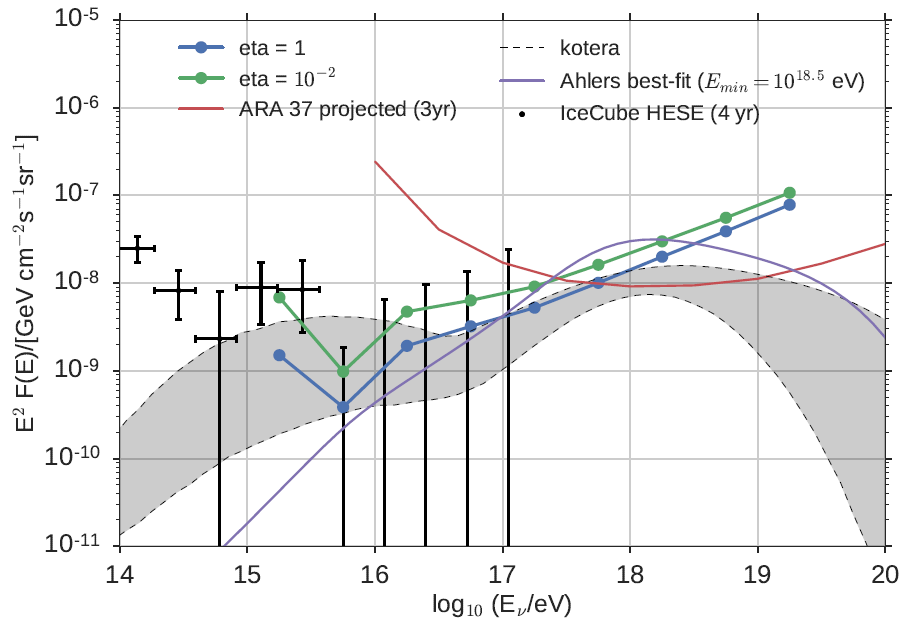
\includegraphics[keepaspectratio,width=13cm]{radar}
\end{center}
\colorbox{yellow}{Radar reflections from shower plasma}\\
New idea (VUB) for $E<10^{17}$ eV\\
{\blue Fill IceCube-Radio $E$ gap}

\Tr
\onecolumn
\begin{center}
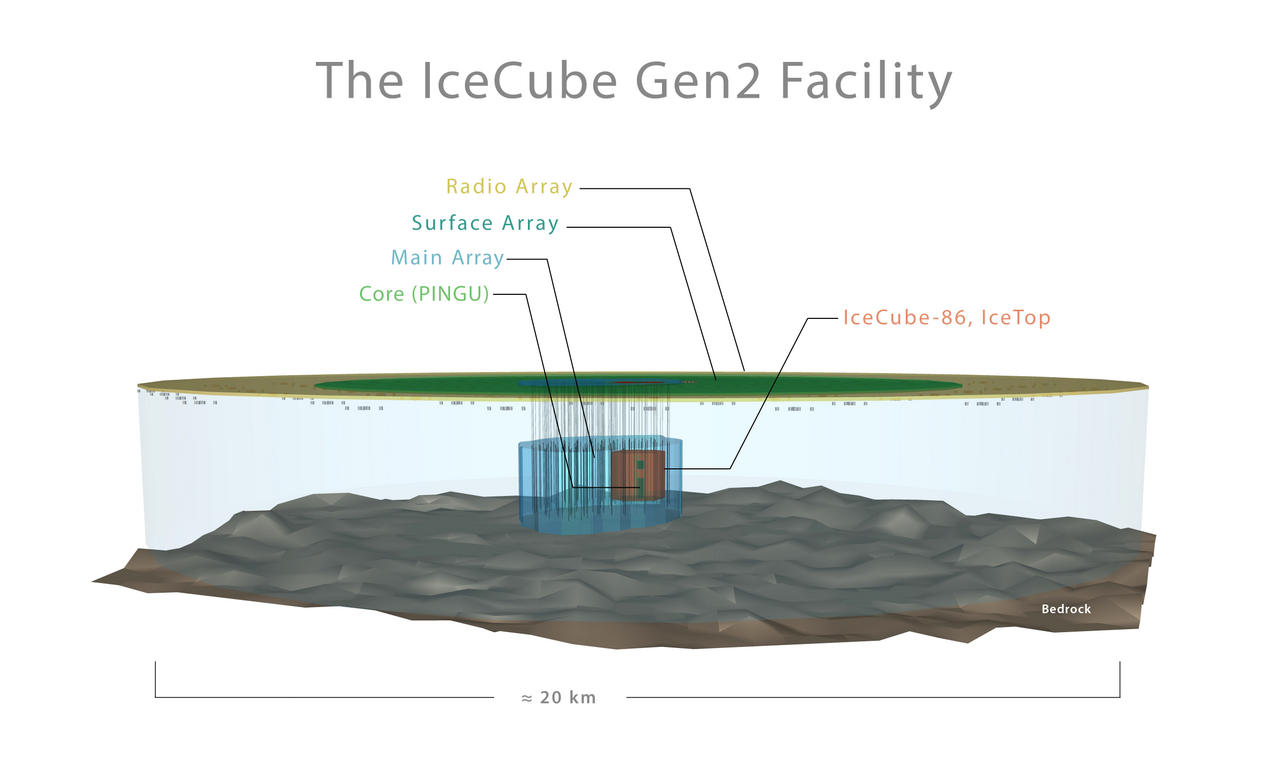
\includegraphics[keepaspectratio,height=15cm]{icecube-gen2}
\end{center}

\Tr
\onecolumn
\begin{center}
{\blue IceCube has now really opened the area of Neutrino Astronomy !}\\[3mm]
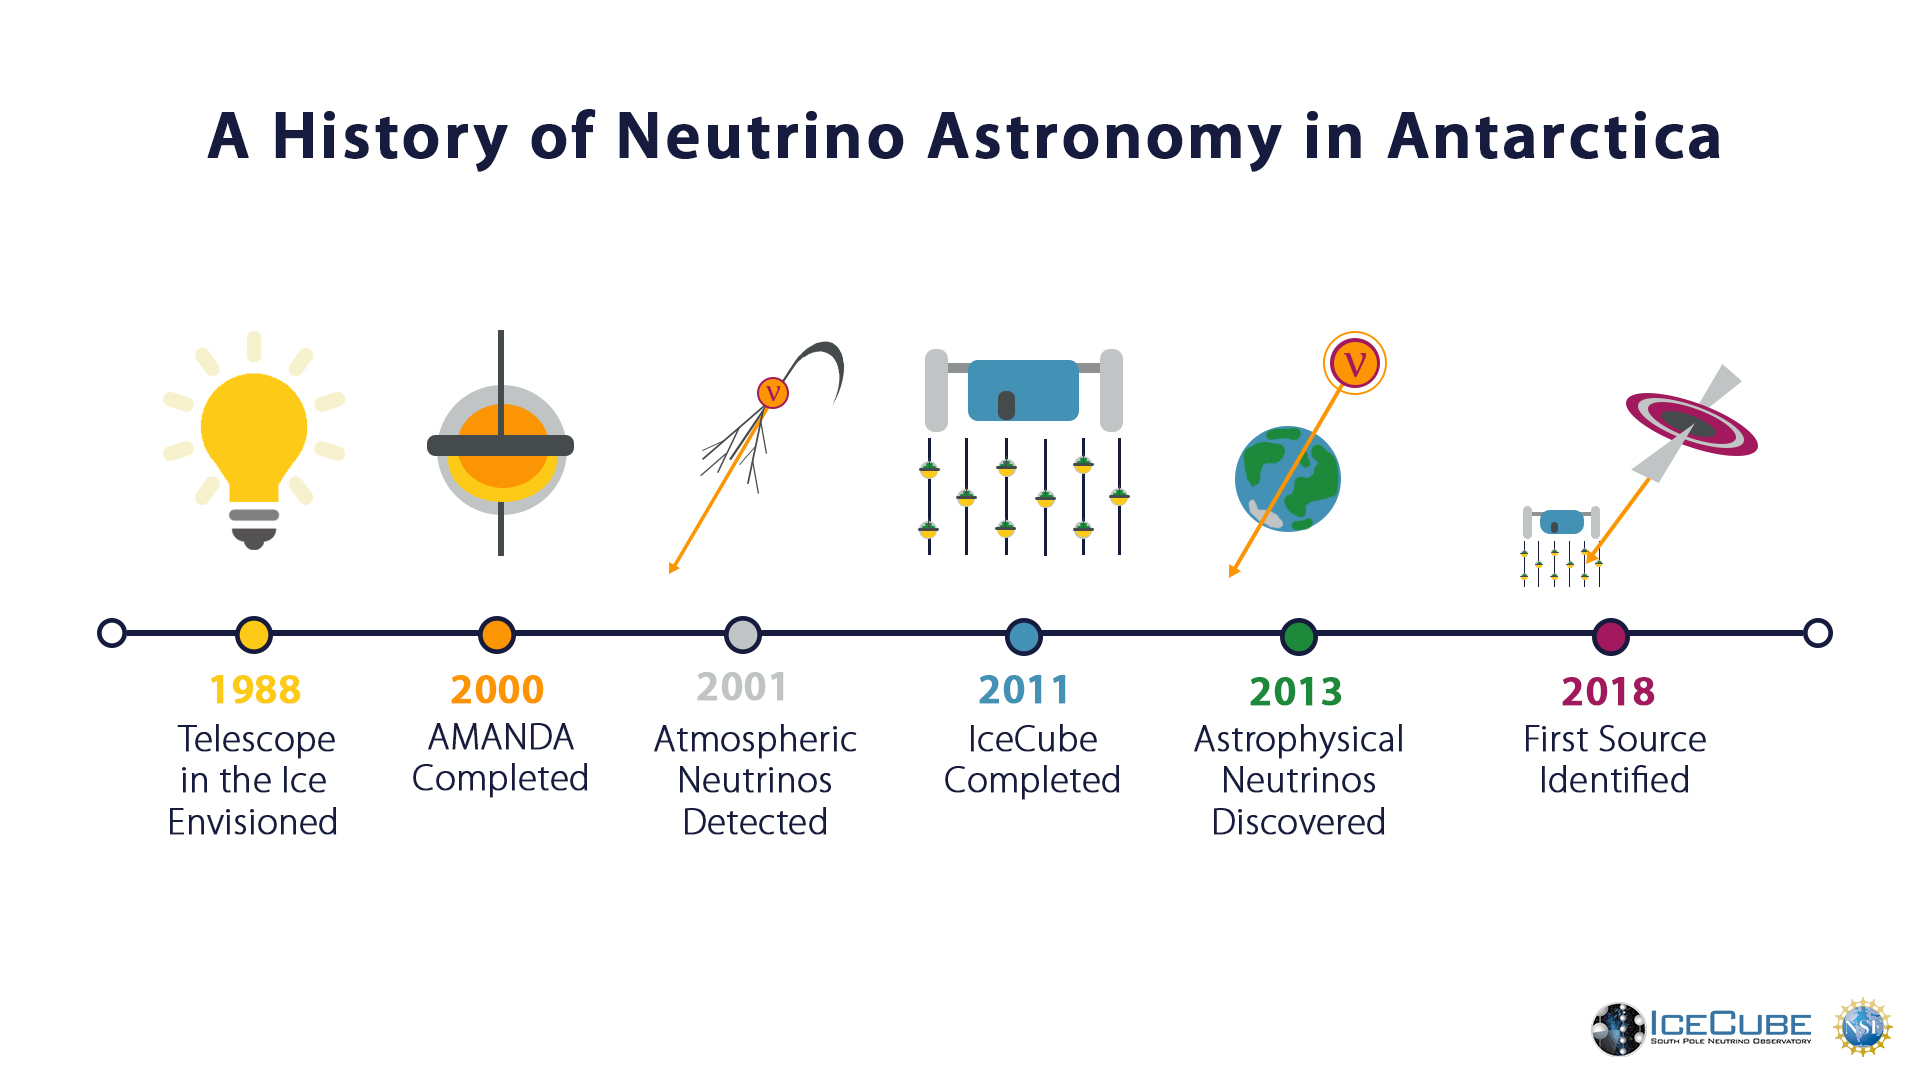
\includegraphics[keepaspectratio,width=26cm]{IC-timeline}
\end{center}

\Tr
\onecolumn
\begin{center}
{\blue The curtain has been raised.......}\\[5mm]
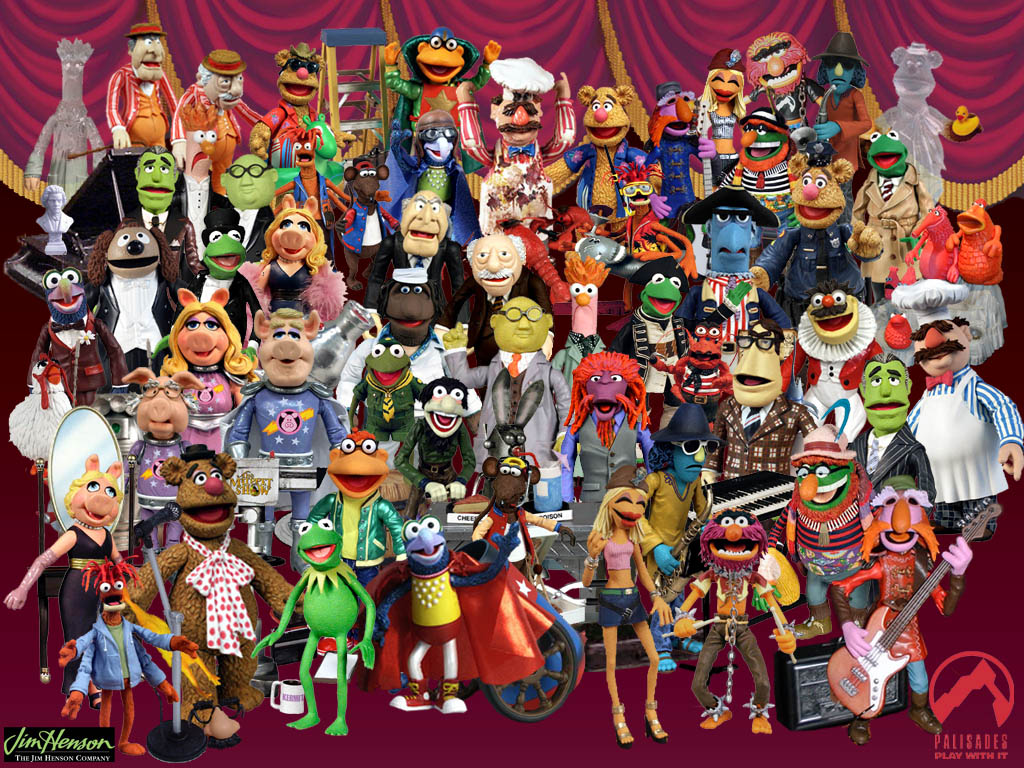
\includegraphics[keepaspectratio,width=18cm]{muppets}\\
\colorbox{yellow}{Let the show begin !}
\end{center}
